%Helper file which allows me compile the article without worrying about ABNT stuff

\documentclass[12pt]{article}
\usepackage[a4paper,top=25mm,bottom=25mm,width=150mm]{geometry}
\usepackage[brazilian]{babel}
\usepackage[backend=biber,style=authoryear,sorting=nyt]{biblatex}
\usepackage{datetime}
\addbibresource{refs.bib}

\usepackage[T1]{fontenc}
\usepackage[utf8]{inputenc}

\usepackage{listings}
\usepackage{graphicx}
\lstset{language=Python,
  basicstyle=\ttfamily\scriptsize}

\newcommand{\figblocks}{
\begin{figure}
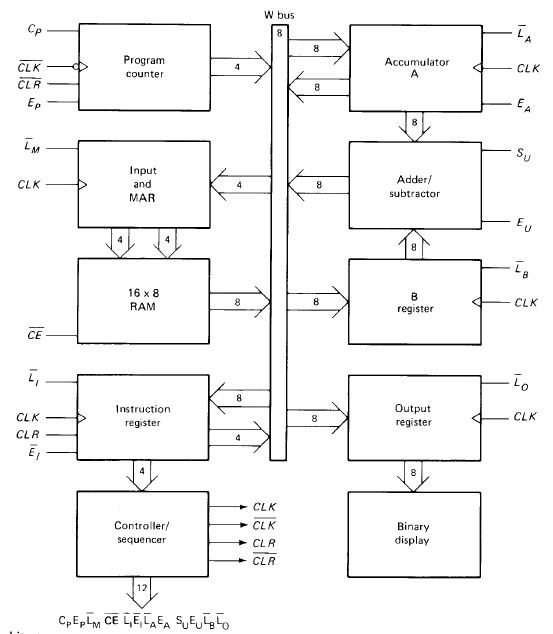
\includegraphics[width=0.6\linewidth]{figures/blocks.jpg}
\caption{Diagrama de blocos do processador SAP1. \cite{malvino}}
\label{f-blocks}
\end{figure}
}

\newcommand{\figblockmux}{
\begin{figure}
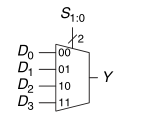
\includegraphics[width=0.5\linewidth]{figures/42-mux.png}
\caption{Bloco representando circuito multiplexador 4:2.}
\label{f-42mux}
\end{figure}
}

\newcommand{\fighmux}{
\begin{figure}
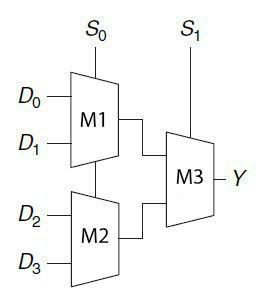
\includegraphics[width=0.5\linewidth]{figures/h-mux.jpg}
\caption{Diagrama de circuito multiplexador 4:2 construido hierarquicamente usando 3 multiplexadores 2:1.}
\label{f-hmux}
\end{figure}
}

\newcommand{\figcd}{
\begin{figure}
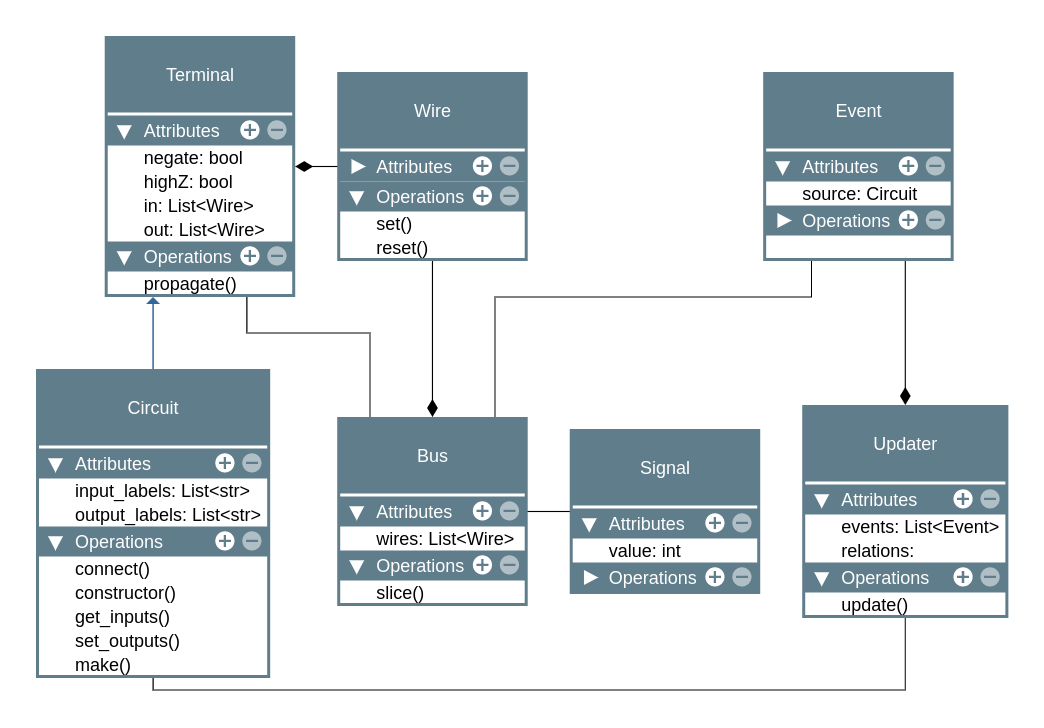
\includegraphics[width=\linewidth]{figures/class-diagrams.png}
\caption{Diagrama de classes para ferramenta.}
\label{f-cd}
\end{figure}
}

\newcommand{\logo}{

\includegraphics[width=0.3\textwidth]{figures/uninter-logo.png}\\
}

\newcommand{\parecer}{
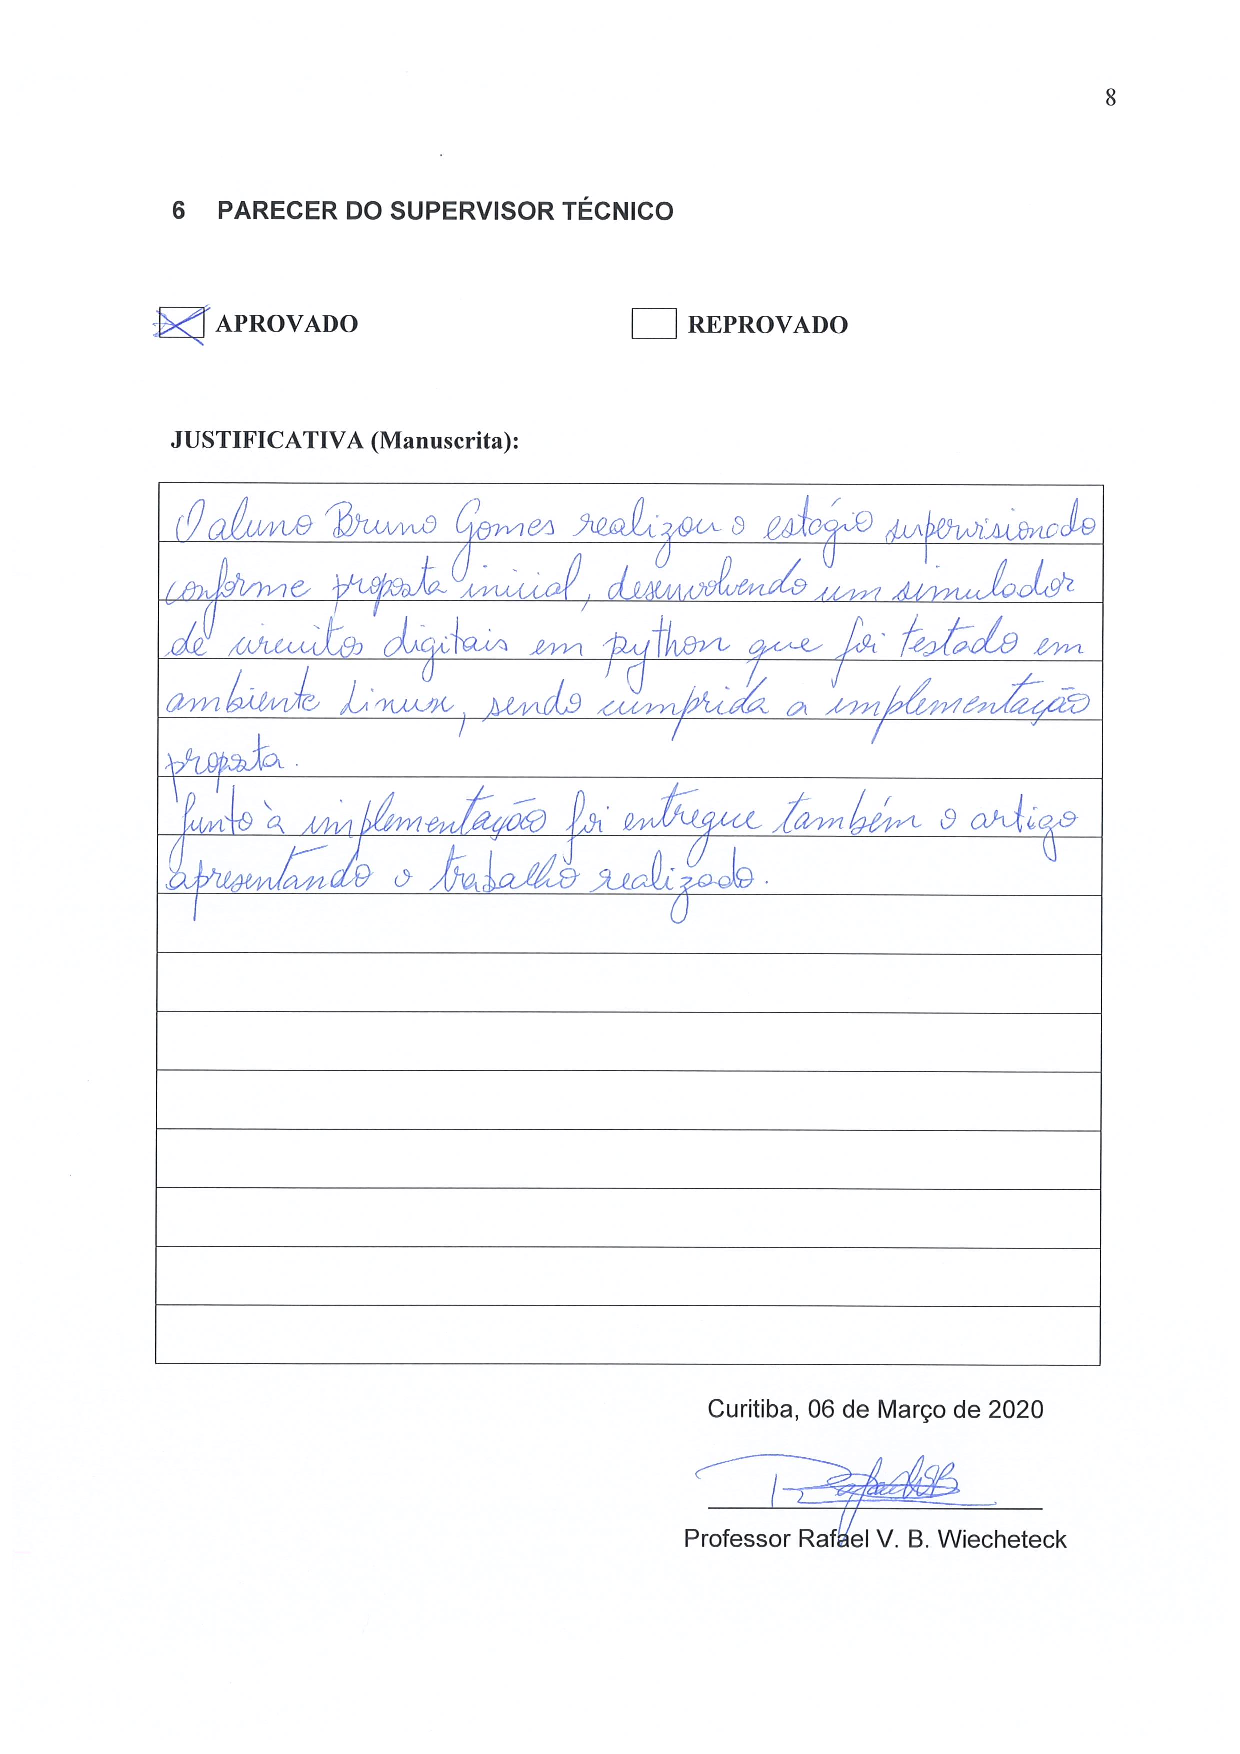
\includepdf[pages=-]{figures/parecer-tecnico.pdf}
}

\renewcommand{\cite}{\parencite}

\newdateformat{mydate}{\THEMONTH \/ \THEYEAR}

\usepackage{pdfpages}

\usepackage{hyperref}
\hypersetup{
  colorlinks,
  citecolor=black,
  filecolor=black,
  linkcolor=black,
  urlcolor=black
}

%Macros 
\newcommand{\disciplina}{disciplina de computação gráfica}
\newcommand{\aluno}{Bruno Gomes}
\newcommand{\prof}{Prof. Marcos Eduardo Pivaro Monteiro}
\newcommand{\cidade}{curitiba}
\newcommand{\estado}{paraná}
\newcommand{\curso}{bacharelado em engenharia da computação}

\begin{document}

\begin{titlepage}
  \begin{center}
    \vspace{0.7cm}
    \textbf{CENTRO UNIVERSITÁRIO INTERNACIONAL UNINTER}\\
    \vspace{0.3cm}
    \textbf{CURSO DE ENGENHARIA DA COMPUTAÇÃO}\\
    \vspace{3cm}
    \logo
    \vspace{2cm}
    \textbf{\MakeUppercase{relatório de estágio supervisionado obrigatório}}\\
    \vspace{5cm}
  \end{center}
\end{titlepage}

\begin{center}
  \MakeUppercase{\cidade}\\
  \mydate \today\\
  \MakeUppercase{\aluno}\\
  \vspace{7cm}
  \textbf{RELATÓRIO DE ESTÁGIO}\\
\end{center}

\begin{minipage}[t]{0.5\textwidth}
\hfill
\end{minipage}
\begin{minipage}[t]{0.5\textwidth}
  \begin{flushright}
  Relatório de estágio apresentado ao Curso de Engenharia de Computação do Centro Universitário UNINTER.
  \end{flushright}
\end{minipage}
  

\newpage
\begin{center}
\MakeUppercase{\cidade}\\
\mydate \today \\
\end{center}
\tableofcontents

\newpage
\section{APRESENTAÇÃO DA EMPRESA}
O Grupo Educacional Uninter é o grupo fundador do Centro Universitário Internacional Uninter.
O Centro Universitário Uninter é uma instituição de ensino superior focada na modalidade de ensino a distância (EaD).
O Centro Universitário se destaca por ter recebido a nota máxima do MEC na modalidade de EaD.


\newpage
\section{HISTÓRICO DA EMPRESA}
O grupo UNINTER nasceu em 1996 e está presente até os dias de hoje.
Durante essa jornada o grupo esteve em constante inovação e mudou sua área de atuação diversas vezes.

Criado em 1996, originalmente conhecido como Instituto Brasileiro de Pós-Graduação e Extensão (IBPEX), fundado pelo professor Wilson Picler, a instituição ofertava cursos de pós-graduação presencial.
No ano de 2000, o grupo expandiu seu mercado e criou a Faculdade Internacional de Curitiba (FACINTER) e começou a ofertar cursos de graduação.
Em 2003, o grupo tomou seus primeiros passos para introduzir a modalidade EaD ao seu repertório e em 2004 foi fundada a Faculdade de Tecnologia Internacional (FATEC) para a oferta de cursos tecnológicos.

Em 2012, o grupo deu um grande salto e fundiu a FATEC e a FACINTER para criar o  Centro Universitário Internacional UNINTER.
Essa nova instituição recebeu o título de Centro Universitário o que lhe permitiu mais autonomia do MEC.

Atualmente, a UNINTER continua se expandindo e vem expandindo o número de cursos ofertados pelo grupo.

\newpage
\section{ATIVIDADES DESENVOLVIDAS}
\section{INTRODUÇÃO}
Qualquer estudante ou profissional que esteja envolvido no ambiente da tecnologia da informação certamente já teve contato com alguma espécie de linguagem de programação em algum ponto de sua jornada.
De acordo com uma pesquisa feita pelo StackOverflow, as 5 linguagens de programação mais usadas são: JavaScript, Python, Java, Linguagens de script (Bash, Powershell, Shell) e C\# \cite{stack-overflow}.

Embora essa lista de linguagens possa parecer como um conjunto heterogêneo de tecnologias, divergindo fortemente em convençoes e nichos de uso, todas essas linguagens fazem parte da família de linguagens conhecidas como imperativas.
Inquestionavelmente, as liguagens imperativas são muito importantes, pois as mesmas compõem a maioria do código sendo produzido diariamente, porém não são a única família de linguagens existentes.
Nesse trabalho será discutido o paradigma de programação funcional, uma alternativa ao paradigma imperativo que domina o mercado.

O foco desse trabalho será a criação de um módulo em Haskell para realizar buscas em textos usando expressões regulares.
Durante essa jornada serão feitas comparações entre algoritmos escritos de maneira imperativa e funcional, usando as linguagens Python e Haskell, respectivamente.
As expressões regulares partem da teoria da computação, mais especificamente da teoria das automatas.
Será definida a teoria as automatas, como elas são capazes de processar expressões regulares e finalemente será abordado a implementação de um módulo em Haskell para a busca em texto.

Embora o paradigma funcional seja muito menos disseminado, ele é de extrema importância e possuem um grande impacto fora de seu nicho. as descobertas e inovações 
Diferentes inovações e descobertas no paradgima funcional, de certo modo infecta as linguagens imperativas.
Como exemplo disso temos que a partir da versão 8 do Java, foram introduzidas interfaces funcionais e \emph{lambda expressions}, conceitos esses que surgiram a programação funcional \cite{java8}.

Em conclusão, embora as linguagem funcionais sejam muito menos comum, elas definitivamente deixaram e continuam deixando marcas nos gigantes da programação.
Elas transcendem seu pequeno nicho de usuários e afetam a grande maioria das pessoas que produzem código regularmente, mesmo que muitos não tenham ciência disso.
Sendo assim, esse trabalho tem como objetivo introduzir o paradigma funcional, através da linguagem Haskell, comparando os dois paradigmas e discutindo a maneira funcional de resolver certos problemas computacionais.

\subsection{REVISÃO DE LITERATURA}
\subsubsection{Características do simulador}
Primeiramente serão definidas as características do simulador, o que também define o escopo do projeto.

O simulador construído faz uso do conceito de hierarquia para construir circuitos.
Segundo \textcite{harris}, hierarquia é um princípio usado para lidar com a complexidade de circuitos digitais, dividindo um sistema em módulos e submódulos até que cada parte seja fácil de entender.
Ainda segundo \textcite{harris}, esse mesmo princípio é usado em linguagens HDL para descrever um circuito de maneira estrutural.

Os circuitos digitais têm uma forte correlação com a lógica matemática.
Essa relação é graças ao conceito de \emph{static discipline}, que restringe os valores de voltagem que um circuito interpreta a duas possibilidades \cite{kaufman}.
Sendo assim, os circuitos digitais fazem uso dos operadores lógicos AND, OR, XOR e NOT.
Esses operadores têm os seus equivalentes na forma de portas lógicas na eletrônica digital.
O simulador disponibiliza as portas AND, OR e XOR como parte da biblioteca.
As portas lógicas são os átomos da eletrônica digital e circuitos mais complexos são implementados a partir delas usando o conceito de hierarquia.

Circuitos digitais reais possuem atrasos e são sujeitos a ruídos \cite{kaufman}.
Esses fatores são de grande preocupação para a construção de circuitos digitais reais e ferramentas HDL levam em consideração essas variáveis.
O simulador ignora essas condições e trabalha com sinais digitais perfeitos (sem ruído) e instantâneos (sem atraso).
Essa simplificação possibilita uma ferramenta menos complexa e mais amigável.

Uma grande vantagem da HDL é que ela pode ser usada para simulação e síntese de circuitos.
O processo de síntese da HDL realiza simplificação de portas lógicas e realiza otimizações para o tipo de tecnologia que será usada no processo de fabricação \cite{harris}.
A ferramenta construída não realiza o processo de síntese ou de simplificação de portas lógicas.

O simulador faz uso da orientação a objetos para construir circuitos e foi definido um modelo que descreve circuitos usando classes.
Para criar um circuito o usuário deve escrever uma classe e especificar os sub-circuitos e as ligações entre eles.
As classes criadas podem então ser usadas para a criação de outro circuitos, fazendo uso do conceito de hierarquia.

O processo de simulação será feito através de scripts ou via um interpretador.
A interação via interpretador é mais simples porém limitada e repetitiva.
A vantagem é que o interpretador é um ambiente interativo com feedback instantâneo que ajuda no processo criativo.
Os scripts consistem de: inicializar o circuito a ser simulado e variar os sinais de entrada desse circuito.
Assim, o usuário pode usar um script para gerar a tabela verdade do circuito que ele criou e verificar se o mesmo esta correto.
O uso de scripts pode parecer desnecessariamente complicado porém apresenta a vantagem de ser automatizável, sendo possível automatizar o processo de teste e simulação de circuitos usando funções. 

\subsubsection{Eletrônica digital em objetos}

O objetivo dessa seção é: apresentar o paradigma orientado a objetos, identificar os constituintes da lógica digital e definir quais objetos farão parte do modelo que irá ser usado pela ferramenta. 

A programação orientada a objetos parte do princípio de criar um modelo, em software, um sistema físico.
Esse paradigma é explicado por \cite{objects} como:

\begin{quote}
O paradigma de orientação a objetos é baseado em uma correlação intuitiva entre um software simulando um sistemas físico e o sistema físico propriamente dito.
É feita uma analogia entre construir um modelo algorítmico de um sistema físico a partir de componentes de software e construir um modelo mecânico do sistema a partir de objetos concretos.
Sendo assim, por analogia, os próprios componentes de software passam a ser chamados de objetos.
\end{quote}

A orientação a objetos facilita a macro visão, pois o mesmo passa a ser mais concreto e modular.
Deseja-se criar um modelo orientado a objetos para circuitos digitais que seja intuitivo para o usuário.
Para construir um modelo orientado a objeto é necessário identificar o que seriam os objetos que regem a lógica digital.

A literatura define um circuito, no escopo da eletrônica digital, como sendo "[...] uma rede de processamento de variáveis com valores discretos.", \cite{harris}.
Como um circuito é uma rede isso implica que exista comunicação entre os elementos dessa rede.
Em circuitos digital, tal como em circuitos analógicos, os fios são os objetos que transmitem informação entre os elementos.
Essa definição expõe necessidade da existência dos objetos fio e circuito na eletrônica digital, ambos farão parte do modelo de software da ferramenta.

Como visto, fios são os propagadores de informação.
Cada fio contém uma unidade de informação, chamado de bit.
Alguns circuitos recebem múltiplos bits de informação, tal como um somador de 8 bits.
Naturalmente o aumento do número de bits sendo transmitido aumenta o número de fios.
É desejável abstrair essa característica.
Na literatura, um grupo de fios carregando partes da mesma informação para um circuito são agrupados e denominados de Bus.
Como um fio transmite um bit uma bus transmite vários bits.
Um grupo de bits será denominado de sinal.
Isso introduz dois novos objetos: bus e sinal.

O objeto sinal é um pouco peculiar por não ter um equivalente preciso em um circuito físico, vendo que pode-se apenas medir o sinal (voltagem) de apenas um fio de cada vez.
O objeto sinal é um exemplo de uma abstração definida a fim de simplificar o modelo.
Para o usuário, é mais conveniente representar uma Bus como um único número, ao invés de um conjunto de bits.
O sinal é construído a partir desse conjunto de bits que são interpretados como um número binário.
De maneira geral, o sinal de uma bus com $n$ fios é um número natural no intervalo $[0,2^n -1]$, onde $n \in N $ \cite{harris}.

Foi visto o que um circuito faz mas não sua interface.
Segundo \textcite{harris}, o circuito é como uma caixa preta que contém terminais de entrada, terminais de saída, uma função que computa a saída a partir das entradas e uma especificação de atrasos no circuito.
Internamente um circuito contém fios e elementos, onde elemento se refere à outros circuitos \cite{harris}.
Essa definição introduz um novo elemento, o objeto terminal.
Pode-se considerar os terminais de entrada e saída como sendo a interface de um circuito, pois definem como interagir com o mesmo.
Essa definição esta de acordo com \textcite{kaufman}, onde é dito que "[...] o acesso à circuitos eletrônicos é feito por terminais.".
A partir das definições acima pode-se entender que terminais separam a parte interna e externa de um circuito, em termos de classes, podemos dizer que circuitos contém objetos terminais e que terminais estão associados a um conjunto de fios, ou seja uma Bus.

Em conclusão, circuitos digitais são compostos por: fios, terminais e circuitos.
Cada fio armazena uma unidade de informação, um bit, que é transmitida a outros circuitos através de terminais neles.
Uma abstração que ocorre naturalmente na disciplina é agrupar um conjunto de fios e denominá-los de Bus, buses possuem um sinal.
Os objetos que devem ser codificados então são: fio, bus, terminal e circuito.

\subsubsection{Construção do simulador}

O processo de construção do simulador envolve traduzir as relações descritas na seção anterior para a linguagem de software.
Esse processo formalmente é feito usando diagramas UML.
A fígura \ref{f-cd} formaliza o modelo criado tal que ele possa ser transformado em software.
A fígura especifica a relação entre as classes do software usando a notação tradicional das linguagens UML.
Dentre elas: Buses possui Wire, Signal é associado a Bus, Terminal é associado a Bus e Circuit possui Terminal.

\figcd

Embora tenha sido definido um modelo de software para circuitos digitais, esse modelo está incompleto.
Como foi visto, circuitos digitais são uma rede de processamento de variáveis.
Ao modificar a entrada de um circuito, isso modifica a saída do mesmo.
No caso da saída estar conectada, existe a necessidade de atualizar o circuito encadeado.
Uma solução para isso seria atualizar todos os objetos circuitos cada vez que um sinal seja alterado, mas isso é um enorme desperdício.
Sendo assim, é necessário um componente em software que atualize somente os circuitos afetados.

O simulador faz uso de eventos e um objeto auxiliar para orquestrar o processo de atualização de circuitos.
Essa solução é um padrão de projeto conhecido como \emph{Observer}.
O intuito desse padrão é "definir uma dependência de um-para-muitos entre objetos tal que quando um objeto mude de estado, todo seus dependentes sejam notificados e atualizados automaticamente." \cite{gof}. 

\fighmux

Contextualizando, suponha o circuito da fígura \ref{f-hmux}, um circuito multiplexador 4:2 feito a partir de 3 multiplexadores 2:1.
Nota-se que o circuito possui 6 entradas e 1 saída.
Suponha que o sinal no terminal D0 seja modificado, a bus D0 está ligada somente ao circuito M1 e nenhum outro, seria um enorme desperdício se o simulador recalculasse a saída de todos os circuitos do programa.
Fica aparente a necessidade de uma entidade que controle quais circuitos devem ser atualizados a cada alteração de sinal e foi nesse sentido que foi utilizado o padrão Observer.


\subsubsection{Processador SAP1}
\paragraph{Arquitetura SAP1}
Parte do projeto envolve a construção de um processador.
Existem inúmeras arquitetura didáticas que poderiam ser implementadas porém foi escolhido a arquitetura SAP1.
Nessa seção será apresentado os aspectos principais dessa arquitetura.

A arquitetura SAP1 é uma arquitetura de 8 bits com um conjunto de instruções mínimo.
Essa arquitetura é apresentada por \cite{malvino}.
Embora contenha um conjunto de instruções reduzido ela apresenta os elementos comuns a todas arquitetura, tais como registradores, unidade de controle, ALU, MAR e etc.
Essa arquitetura foi escolhida por ter um balanço entre um conjunto de instruções simplificado e microarquitetura moderadamente realística.

A fígura \ref{f-blocks} apresenta um diagrama de blocos da arquitetura.
Notam-se dois registradores conectados ao somador (A e B), um registrador de saída (O), banco de memória de 16x8 e os demais componentes esperados como registrador de endereço de memória (MAR), contador de programa (PC) e unidade de controle (CU).
Essa arquitetura apresenta uma única bus (W) que é usada para transmitir endereços e dados, para que não haja sobreposição de valores em W a arquitetura faz uso de lógica de três estados.

\figblocks

O conjunto de instruções da arquitetura é apresentado de maneira resumida na tabela \ref{t-inst}.
Essas instruções são: ADD, LDA , SUB e HLT, porém a instrução HLT foi omitida na construção do processador por ser redundante.
É importante destacar que essa arquitetura não apresenta nenhuma instrução de jump, o que limita muito o tipo de computação que pode ser feito.
Todas as instruções dessa arquitetura seguem o mesmo formato, 8 bits de comprimento sendo os bits $[0,3]$ destinados à endereço ou dado e os bits $[4,7]$ sendo reservados para o OP code da instrução.
Em seguida serão abordado os funcionamentos de cada instrução.

\begin{table}
  \caption{Instruções da arquitetura SAP1 e suas descrições.}
\begin{tabular*}{0.5\linewidth}{lcp{4cm}}
  \hline
 Inst. & Op code & Descrição \\
 \hline
 LDA         &     0x0 & Carrega o acumulador com o valor contido nos bits [0,3] \\
 ADD         &     0x1 & Soma o valor presente no acumulador com o valor contido no endereço apontado pelos bits [0,3] da instrução. \\
 SUB         &     0x2 & Subtrai o valor presente no acumulador com o valor contido no endereço apontado pelos bits [0,3] da intrução.\\
 OUT         &     0xE & Escreve o valor contido no acumulador ao registro de saída (O). \\ 
 \hline
\end{tabular*}
\label{t-inst}
\end{table}


A instrução LDA é utilizada para carregar um valor ao registrador A.
Essa instrução contém nos 4 primeiros bits um endereço que será acessado pelo MAR e o valor contido na memória é carregado no registrador A.
Um exemplo da instrução LDA em linguagem de máquina é 0x19, ou seja, carregar o valor contido no endereço 9 no registrador A.

As instruções ADD e SUB possuem um funcionamento análogo porém realizam operações matemáticas diferentes, essas instruções somam e subtraem, respectivamente, o valor armazenado no registrador A ao valor carregado no registrador B.
Elas possuem em seus 4 primeiros bits um endereço de memória cujo valor é armazenado é copiado ao registrador B.
A ALU então opera sobre os registradores A e B e o resultado dessa operação é armazenado no registrador A.
Um exemplo dessa instrução em linguagem de máquina seria 0x25, ou seja, carregar o valor no endereço 5 ao registrador B, somar os valores de A e B e armazenar o resultado em A. 

A instrução OUT é extremamente simples, ela copia o valor contido no registrador A para o registrador O.

O processador possui 3 registradores disponível ao usuário: registrador A, registrador B e registrador O.
O registrador A funciona como acumulador e após as instruções de soma (SUM) e subtração (SUB) o resultado da operação é armazenado nele; é possível também alterar diretamente o valor de A utilizando a instrução LDA que carrega o valor contido no endereço encodado na instrução a ele.
O registrador B funciona como um registrador auxiliar para as instruções de SUM e SUB.
O endereço indicado pelas instruções é acessado e o valor contido nele é carregado ao registrador B.
O valor do registrador B é alterado a cada instrução de SUM ou SUB.
Finalmente, o registrador O é utilizado para apresentar informação ao usuário.

\paragraph{Micro arquitetura}
Uma importante característica da micro arquitetura do SAP1 é que ela possui micro instruções.
A micro arquitetura construída foi fortemente baseada na implementação feita na literatura.
A característica principal dessa microarquitetura é que todas as instruções são executadas em 6 pulsos do clock.
\footnote{Os detalhes dos ciclos das micro instruções são desnecessários para a construção do processador e para a compreensão da arquitetura da perspectiva do programador. A explicação completa do funcionamento dessa arquitetura pode ser encontrado na obra citada.}

As conexões entre os componentes do processador podem ser visualizados na imagem \ref{f-blocks}.
Como mencionado anteriormente, essa arquitetura usa lógica de três estados para preservar o valor escrito em W.
Os blocos PC, RAM, IR e A apresentam lógica de três estados na saída e os blocos A, B, O, IR e MAR apresentam lógica de três estados nos terminais de entrada.
O controle dos blocos é regida pelas 12 flags presentes na imagem.
A tabela \ref{t-flags} apresenta o propósito dessas flags. 

\begin{table}
  \caption{Descrição das flags de controle do processador.}
\begin{tabular}{ll}
\hline
Flag & Descricao \\
\hline
cp & Incrementar PC no proximo clk \\
ep & Tristate de saida do PC \\
lm & Tristate de entrada do MAR \\
ce & Tristate saida da RAM \\
li & Tristate de entrada do IR \\
ei & Tristate de saida do IR \\
la & Tristate de entrada do acumulador \\
ea & Tristate de saida do acumulador \\
su & Flag de subtracao para o adder/subtractor \\
eu & Tristate de saida para o adder/subtractor \\
lb & Tristate de entrada para o registrador B \\
lo & Tristate de entrada para o registrador output \\
\hline
\end{tabular}
\label{t-flags}
\end{table}


A literatura apresenta duas alternativas para a construção da unidade de controle (CU), uma baseada em lógica combinacional e a outra em uma memória ROM.
Foi escolhido a CU que utiliza memória ROM por ser mais simples de implementar no simulador.
Essa CU possui dois terminais de entrada, IW (palavra de instrução) e MIW (palavra de micro instrução) e um de saída CW (palavra de controle).
A entrada IW carrega os 4 bits que representam o opcode da instrução sendo executada e a entrada MIW contém o ciclo de micro instrução (número de 0 a 5 gerado pelo MIC).
A saída CW é uma bus de comprimento 12 que orquestra os blocos do processador, essas flags são utilizadas para controlar o comportamento dos registradores, CU e lógica de três estados.
Como explicado acima, essa CU é uma lookup table para produzir as flags das micro instruções.
O endereço da memória é dado pela concatenação das buses IW e MIW.

\subsection{METODOLOGIA}

Como explicado na introdução, o foco destre trabalho é demonstrar alguns  elementos da programação funcional.
Para isso, foi escolhido o problema de implementar um módulo de busca de strings usando expressões regulares.
Será escolhido trechos de código especialmente interessante do módulo escrito que serão explciados a fundo.

Foi visto que uma expressão regular pode ser convertida em uma automata equivalente.
Sendo assim, o problema possui duas tarefas: criar submódulo para converter uma regex em uma automata e implementar um submódulo que permita criar e operar uma automata.
Serão definidas as arquiteturas de cada submódulo tal como o encadeamento de funções que serão chamadas para resolver cada problema, análogo ao que foi feito anteriormente.
Será explicado, de maneira alto nível, o que cada função faz baseada em suas entradas e saídas.
Isso irá motivar a introdução de tipos de dados únicos a programação funcional.

Além dessa inspeção de "caixa preta" das funções, os pontos principais do módulo será explicado em detalhe, o que permitirá aa análise de conceitos importantes no paradigma funcional.
Será feita uma comparação entre trechos escrito de maneira funcional e imperativa.
Essa comparação tem dois objetivos: introduzir conceitos referentes a linguagem funcional e identificar em quais situações um código funcional é mais simples, ou mais complexo, que o seu equivalente de maneira imperativa.
Para introduzir os conceitos do paradigma funcional, o código irá ser projetado tal que demonstre as diferentes ferramentas que compõe a caixa de ferramentas de um programador funcional.
As ferramentas simples abordarão conceitos comos imutalidade e recursão e as ferramentas mais complexas irão introduzir abstrações muito perculiares da programação funcional tal como \emph{Functors} e \emph{Applicative Functors}.
A metodologia escolhida tem como objetivo ser transparente quanto aos lados bons e ruins da programação funcional e também auxiliar a associação do paradigma imperativo ao funcional.
Dessa forma, um leitor familiar com programação imperativa poderá entender como um problema resolvido de maneira imperativa pode ser traduzido para um algoritimo funcional.

Em conclusão, o trabalho irá resolver o problema de criar um módulo de procura em texto usando expressões regulares.
O problema será quebrado em funções, exemplificando como resolver um problema a partir de funções ao invez de passos.
O código fonte do módulo criado será usado para introduzir conceitos sobre o paradigma funcional e familiarizar o leitor com algumas ferramentas.
Ao mesmo tempo, trechos de códigos funcionais serão comparados com seu equivalente escrito em uma linguagem imperativa, o que permitira associar conceitos imperativos a funcionais e expor os pontos fortes e fracos desse paradigma.

\subsection{ANÁLISE E DISCUSSÃO}
A ferramenta criada modela os circuitos digitais de uma maneira simplificada.
Circuitos são compostos de terminais de entrada e saída,  sub circuitos internos e uma rede de ligações.
Esse modelo implementado usando orientação a objeto resultou em uma descrição simplificada de um circuito.
Essa descrição faz com que a curva de aprendizado da ferramenta seja, teoricamente, pequena.

A utilização da hierarquia como parte do processo de construção dos circuitos resulta em circuitos modulares.
Isso é de grande vantagem pois facilita a interoperabilidade dos circuitos escritos por um ou mais usuários.
Assim, caso o usuário deseja construir um circuito complexo, a modularidade permite que ele separe a construção do circuito em módulos.
Trabalhar em módulos elimina repetição e permite que cada modulo seja testado isoladamente, fazendo uso de testes unitários.

Como foi visto, um requisito do simulador é que ele fosse capaz de simular um processador.
Usando a ferramenta, foi possível construir o processador e o mesmo produziu os resultados corretos. 
A modularidade facilitou muito no processo de construção pois cada modulo foi testado individualmente antes de serem unidos.
A construção do processador foi simples e resultou em um número moderado de linhas de código, foram menos de 40 linhas para conectar todos os módulos do processador.

O código do processador foi testado usando os programas descritos na seção anterior.
A execução correta desses programas demonstra que todas as instruções do processador funcionam adequadamente.
O snippet abaixo demonstra o resultado impresso no terminal para a simulação dos programas 1 e 2.
Observa-se que o valor de saída (out) para o programa 1 e 2 estão de acordo com o esperado, como foi descrito na metodologia.

\begin{lstlisting}
~/projects/pdd/builds/sap1 $ python run.py 
Tempo de execucao: 0:03:29.625620
resultado prog. 1 Processor: {'clk': '0x0', 'r': '0x0', 'out': '0x3', 'wout': '0x4'}
resultado prog. 2 Processor: {'clk': '0x0', 'r': '0x0', 'out': '0x7', 'wout': '0xe4'}
\end{lstlisting}

Um ponto negativo da metodologia textual usada é que para um circuito complexo como o processador, traçar as conexões é algo complexo.
A partir dessa experiência ficou claro que a carência de qualquer forma de representação gráfica do circuito pode ser prejudicial em algumas construções.
Uma possível solução seria adicionar um modulo que gera um diagrama de conexões a partir de um objeto circuito.

Embora exista uma dificuldade não esperada com a interface da ferramenta, existe um problema grave de performance que deve ser corrigido para viabilizar o seu uso.
Isso pode ser observado no tempo de execução dos 2 programas usados para testar o processador.
Cada processador executou menos de 5 instruções no total, a execução dos 2 programas escritos para o processador demorou um tempo inaceitável, 3.5 minutos, aproximadamente.
Essa quantia de tempo é astronômica dado a simplicidade das instruções realizadas.
Deve ser ressaltado que o processador SAP1 usa uma única bus, armazena apenas 16 palavras em memória, opera sobre palavras de 8 bit e possui uma ALU simples.
É passível de concluir que a simulação de um processador mais complexo, como um de 32 bits seria inviável.
Esse problema de performance é devido a metodologia hierárquica usada.

Como o elemento base de todos os circuito construídos no simulador foram as portas lógicas, isso significa que todas as operações do circuito utiliza as operações AND, OR e XOR do computador host.
Isso é um enorme desperdício dos diversos componentes de hardware já presentes no host.
Por questões de eficiência, o simulador poderia estar fazendo uso dos circuitos de operações matemática e memória embutidos no próprio computador.
Embora a construção desse circuitos a partir de portas lógicas seja um processo instrutivo, quando usados em um circuito complexo, isso prejudica a performance do simulador.
A correção desse problema é relativamente simples, basta reescrever as classes de circuitos somadores, subtratores, registradores e etc tal que esses circuitos usem os operadores presentes na linguagem Python.
Por exemplo, de maneira análoga ao que foi feito na classe AND, onde foi usando o operador \&, a classe do circuito somador usaria o operador "+".
Isso evita implementar essa operação usando portas lógicas.

A solução para o problema de performance indiretamente resolve uma outra inconveniência relacionada a inspeção de circuitos sequenciais.
A inspeção de um circuito combinacional pode ser feito de maneira conveniente na ferramenta, pois basta verificar o seus valores de entrada para identificar a saída.
Essa inspeção é feita usando o comando print, que apresentada os sinais de todas os terminais de entrada e saída.
Porém devido a natureza da lógica sequencial, seria interessante manter uma lista dos valores anteriores de um circuito sequencial, sendo assim possível fazer uma análise temporal de um circuito de maneira simplificada.
Por exemplo, suponha a existência de um circuito contador configurável, seria conveniente poder alterar e armazenar um sinal no contador sem alterar o valor na bus do circuito.
Isso permite que seja possível induzir um estado em um circuito sequencial, o que facilita o processo de debug.
Para implementar isso, basta adicionar um método de configuração nos circuitos sequenciais, tal como um circuito FlipFlop. 

Em conclusão, a ferramenta construída provou-se capaz de realizar a simulação de diversos circuitos digitais.
Na construção dela foi utilizado um paradigma orientado a objetos para descrever um circuito, pois acreditava-se que esse paradigma iria simplificar a modelagem de circuitos.
O escopo do projeto foi delimitado para a construção da ferramenta, como consequência não se sabe se esta ferramenta é de fato mais simples para um novato na disciplina.
Um interessante próximo passo seria disponibilizar esta ferramenta em um ambiente web a fim de realizar um teste alfa e receber feedback.
Seria possível desenvolver um webapp com um interpretador Python que contém a biblioteca instalada no ambiente virtualizado.
Essa metodologia de uso seria ideal pois não requer a instalação da biblioteca ou da linguagem Python no computador do usuário.



\newpage
\section{CRONOGRAMA REALIZADO}
\section{CRONOGRAMA REALIZADO}
\section{CRONOGRAMA REALIZADO}
\input{tables/cronograma}



\newpage
\section{CONSIDERAÇÕES FINAIS}
Durante o projeto de estágio foi construído uma ferramenta em Python para simulação de circuitos digitais.
Essa ferramenta faz uso do paradigma de programação orientada a objetos para descrever um circuito.
Sendo assim, a implementação de um circuito é feita a partir de classes codificadas pelos usuários.
Essa metodologia garante circuitos modulares e regulares pois faz uso do conceito de herança para garantir uma interface consistente entre circuitos.

A ferramenta desenvolvida foi utilizada para construir um processador SAP1, uma arquitetura didática.
A ferramenta se mostrou capaz de simular o processador corretamente, porém foi notável um problema de performance.
Esse problema está relacionado a metodologia hierárquica empregada pela ferramenta.
Possíveis soluções para o problema foram abordadas na seção de analise.

O intuito da ferramenta é criar uma descrição simplificada de circuitos para que estudantes possam construir circuitos de maneira simples com o objetivo de facilitar ao processo de aprendizado.
Espera-se que um estudante possa construir um processador, a partir de uma bibliografia, sem que isso seja uma tarefa complexa e longa.
Sendo assim, essa ferramenta tenta substituir, até certo ponto, a construção de um processador em uma breadboard (processo longo) ou em uma linguagem HDL (processo complexo).

\begin{flushright}
\vspace{3cm}
Curitiba\\
\today\\
\vspace{3cm}
\noindent \rule{0.5\textwidth}{0.4pt}\\
Bruno Gomes\\
\end{flushright}

\newpage
\addcontentsline{toc}{section}{6   PARECER DO SUPERVISOR TÉCNICO}
\parecer

\newpage
\printbibliography
\end{document}
